% Este archivo es parte de la memoria del proyecto fin de carrera
% de Manuel López Urbina. Protegida bajo la licencia GFDL.
% Para más información, la licencia completa viene incluida en el
% fichero fdl-1.3.tex

% Copyright (C) 2012 Manuel López Urbina

\chapter{Comentarios finales}
\label{chap:conclusiones}

\section{Presupuesto}


\begin{table}[H]
  \begin{center}
    \begin{tabular}{|p{8cm}|p{2cm}|p{2cm}|p{2cm}|}
      \hline
      \vspace{+0.2in}{\textbf{Descripción}} & {\textbf{Unidades}} & {\textbf{Precio \EUR{}}} & {\textbf{Total \EUR{}}}\\
      \hline
      \vspace{+0.2in}{Surveyor SRV-1 Blackfin Robot} &  \vspace{+0.2in}{1} &  \vspace{+0.2in}{379,8} &  \vspace{+0.2in}{379,8}\\
      \hline
      \vspace{+0.2in}{Router WIFI Xavi 7968} & \vspace{+0.2in}{1} & \vspace{+0.2in}{35} & \vspace{+0.2in}{35}\\
      \hline
      \vspace{+0.2in}{Capturadora de vídeo} & \vspace{+0.2in}{1} & \vspace{+0.2in}{15} & \vspace{+0.2in}{15}\\
      \hline      
      \vspace{+0.2in}{Cámara y receptor inalámbrico} & \vspace{+0.2in}{1} & \vspace{+0.2in}{54} & \vspace{+0.2in}{54}\\
      \hline      
      \vspace{+0.2in}{Gamepad} & \vspace{+0.2in}{1} & \vspace{+0.2in}{10} & \vspace{+0.2in}{10}\\
      \hline      
      \vspace{+0.2in}{Horas de programación} & \vspace{+0.2in}{350} & \vspace{+0.2in}{45/h} & \vspace{+0.2in}{15750}\\
      \hline
    \end{tabular}
  \end{center}
\end{table}

\begin{table}[H]
  \begin{flushright}
    \begin{tabular}{p{8cm}p{2cm}}
      \vspace{+0.1in}\textbf{Total bruto:} &\vspace{+0.1in}{\EUR{16.264,8}}\\
      \vspace{+0.1in}\textbf{I.V.A. \%: } & \vspace{+0.1in}{21\%}\\
      \vspace{+0.2in}\textbf{Total presupuesto:} & \vspace{+0.2in}{\EUR{19.676,00}}\\
    \end{tabular}
  \end{flushright}
\end{table}


\section{Conclusiones}

La elaboración de este proyecto ha resultado muy gratificante a nivel personal. Uno de los motivos principales ha sido la necesidad de trabajar en numerosas áreas de conocimiento entre las que encontramos la programación en los lenguajes C y C++, la robótica y la visión artificial. Algunas de las plataformas mencionadas eran desconocidas al inicio del desarrollo de proyecto y han sido adquiridas tras una amplia labor de investigación y pruebas de desarrollo con diferentes tecnologías como Matlab y Octave sin éxito. Otro de los motivos ha sido la necesidad de continuar con el aprendizaje de conceptos propios de la visión artificial y del reconocimiento de patrones adquiridos mediante la asistencia a asignaturas correspondientes a Ingeniería Informática de segundo ciclo.\\

Entre los elementos desarrollados se destaca:

\begin{itemize}

\item \textbf{Software de procesamiento de imágenes:} escrito en el lenguaje de programación C, utilizando la biblioteca de visión por computador OpenCV. Se han estudiado los principios básicos del procesamiento de imágenes y reconocimiento de patrones aplicados a la visión por computador para construir un sistema software inteligente capaz de controlar un vehículo de manera inalámbrica desplazándose por el entorno actuando según las señales de tráfico existentes. Todo ello en tiempo real.

Ha sido la parte del proyecto en la que más tiempo se ha invertido, el software de reconocimiento de señales de tráfico ha sido obtenido siguiendo una metodología de desarrollo por prototipos habiéndose desarrollado tres prototipos. El algoritmo de clasificación utilizado ha sido el del vecino más cercano. Como datos de entrada se han utilizado las diferentes imágenes de cada uno de los elementos internos de las señales de tráfico dispuestos en columnas y añadidos a la matriz modelos. 

\begin{figure}[H]
  \begin{center}
    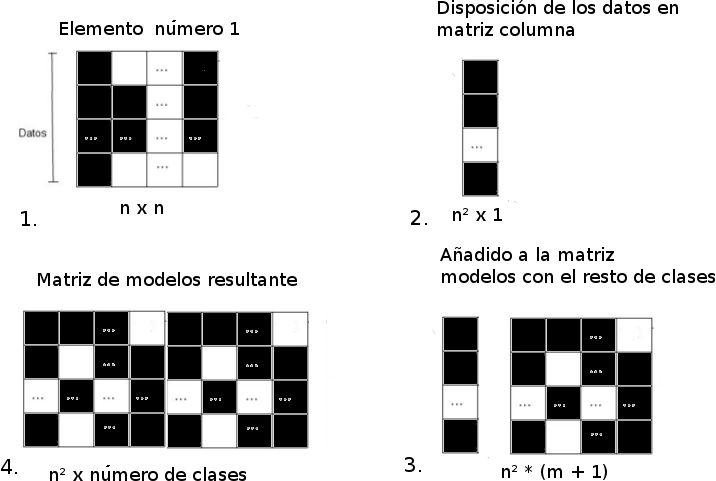
\includegraphics[scale=0.4]{entrenamiento.png}
  \end{center}
  \caption{Pasos para la elaboración de la matriz modelos.}
  \label{fig:com-coche-pc}
\end{figure}


Para la clasificación se ha realizado la comparación de la matriz columna obtenida a partir del elemento desconocido con cada una de las columnas existentes en la matriz de modelos. Cada una de ellas corresponde a una clase. La comparación se realiza mediante el cálculo de todas las distancias euclídeas y quedándonos con la clase que menor distancia ha obtenido, es decir, la más cercana o la que guarda más semejanza. Una vez clasificados todos los objetos internos de una señal de tráfico se evalúa el conjunto y se determina la señal de tráfico resultante.  Los elementos internos son analizados siempre que se encuentren dentro de un contorno rojo o azul y sus formas sean las propias de las señales de tráfico, redondas, octogonales,triangulares o cuadradas.


\item \textbf{Software control del vehículo:} se ha empleado el software denominado \emph{Surveyor Robot Software} desarrollado por la universidad de Brooklyn escrito en el lenguaje de programación C++. El software ha sido adaptado a las necesidades del proyecto. Se ha dotado al vehículo de dos modos de funcionamiento, uno de pilotaje tradicional mostrando las señales detectadas por el software de reconocimiento y otro de pilotaje automático realizado a partir de las señales detectadas.

\item \textbf{Interfaz gráfica:} se ha dotado al conjunto de una interfaz gráfica con la finalidad de proporcionar una experiencia de control al usuario mejorada empleando la biblioteca Qt en C++.

\item \textbf{Sistema de comunicaciones:} el proyecto se compone de dos sistemas de comunicaciones, utilizando cada uno de ellos tecnologías distintas:

\begin{itemize}
\item \textbf{Sistema de comunicaciones WiFi:} hace posible el envío de las órdenes desde el ordenador hasta el coche para su control de forma remota. La comunicación se realiza a través de un router donde se conectan ambos dispositivos, el router y el ordenador, formando una infraestructura de red.

\begin{figure}[H]
  \begin{center}
    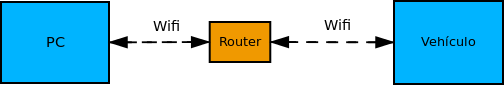
\includegraphics[scale=0.8]{comunicacion-coche-robot.png}
  \end{center}
  \caption{Comunicaciones vía WiFi entre el ordenador y el vehículo robótico mediante un router.}
  \label{fig:com-coche-pc}
\end{figure}

\item  \textbf{Sistema de comunicaciones por radiofrecuencia:} hace posible la recepción de imágenes de vídeo desde la cámara al ordenador de forma inalámbrica. Para hacer esto posible se ha dividido el sistema en tres pasos, primeramente se ha comenzando por la recepción inalámbrica de la imagen emitida por la cámara mediante una receptora de imágenes analógicas. A continuación se realiza una conversión de la imagen de vídeo analógica a digital y finalmente se realiza el envío de la imagen digital al ordenador.

\begin{figure}[H]
  \begin{center}
    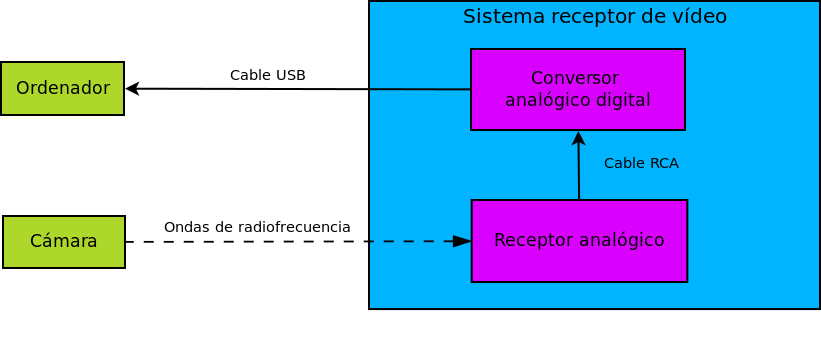
\includegraphics[scale=0.45]{esquema-sistema-receptor-video.png}
  \end{center}
  \caption{Elementos implicados en la transmisión de imágenes desde la cámara hasta el ordenador.}
  \label{fig:com-camara-pc}
\end{figure}

\end{itemize}

 
\end{itemize}

Pienso que el resultado final del proyecto es ideal para aquellas personas aficionadas a la robótica y programación proporcionando una herramienta sea utilizable por la gran comunidad poseedora del vehículo SRV-1 Surveyor en todo el mundo haciéndoles pasar unos momentos divertidos utilizando el vehículo.\\

Una vez presentado podré continuar añadiendo mejoras y muchas cosas que tengo pensadas y que, posiblemente, se realicen para el proyecto de la Ingeniería Informática que me encuentro realizando en la actualidad.

\section{Mejoras futuras}

La aplicación puede mejorarse en diversos aspectos. A continuación, se citan algunas de las mejoras que pueden llevarse a cabo:

\begin{itemize}

\item Incorporación de advertencias acústicas tras la detección de una señal de tráfico.

\item Mejora del diseño de la interfaz gráfica.

\item Permitir la redefinición de las teclas de control del teclado y mando.

\item Permitir la redefinción de la dirección ip en la aplicación en caso de que el vehículo tenga configurada otra dirección ip diferente a la prefijada.

\item Permitir la introducción de nuevas señales detectables al gusto del usuario.

\item Permitir la programación de respuestas al vehículo a señales de tráfico incorporadas por parte del usuario.

\item Mejora del algoritmo de reconocimiento.

\item Mejorar el funcionamiento del algoritmo en situaciones de elevada oscuridad.

\item Adaptar la aplicación al funcionamiento de la cámara que incorpora el vehículo sin la utilización de una cámara independiente empleada debido al estado defectuoso de la original.

\end{itemize}


